% Created by tikzDevice version 0.10.1 on 2017-09-05 00:50:56
% !TEX encoding = UTF-8 Unicode
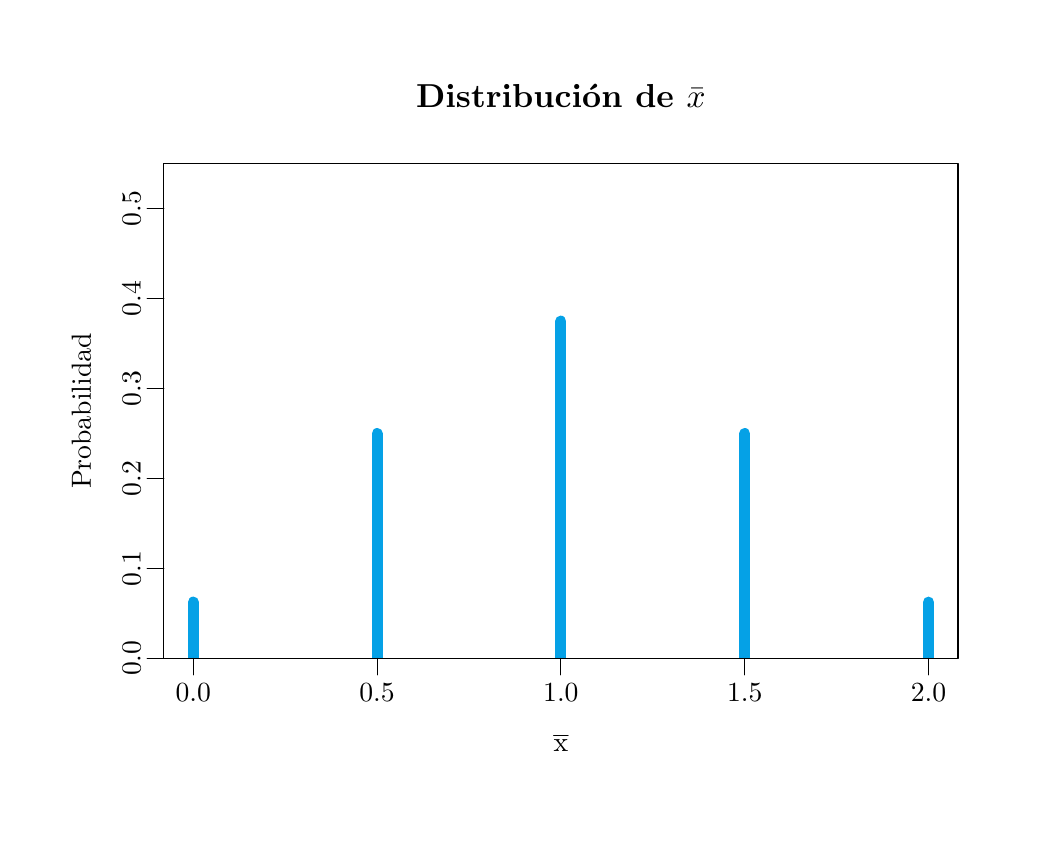
\begin{tikzpicture}[x=1pt,y=1pt]
\definecolor{fillColor}{RGB}{255,255,255}
\path[use as bounding box,fill=fillColor,fill opacity=0.00] (0,0) rectangle (361.35,289.08);
\begin{scope}
\path[clip] ( 49.20, 61.20) rectangle (336.15,239.88);
\definecolor{drawColor}{RGB}{5,161,230}

\path[draw=drawColor,line width= 4.0pt,line join=round,line cap=round] ( 59.83, 61.20) -- ( 59.83, 81.50);

\path[draw=drawColor,line width= 4.0pt,line join=round,line cap=round] (126.25, 61.20) -- (126.25,142.42);

\path[draw=drawColor,line width= 4.0pt,line join=round,line cap=round] (192.67, 61.20) -- (192.67,183.03);

\path[draw=drawColor,line width= 4.0pt,line join=round,line cap=round] (259.10, 61.20) -- (259.10,142.42);

\path[draw=drawColor,line width= 4.0pt,line join=round,line cap=round] (325.52, 61.20) -- (325.52, 81.50);
\end{scope}
\begin{scope}
\path[clip] (  0.00,  0.00) rectangle (361.35,289.08);
\definecolor{drawColor}{RGB}{0,0,0}

\path[draw=drawColor,line width= 0.4pt,line join=round,line cap=round] ( 59.83, 61.20) -- (325.52, 61.20);

\path[draw=drawColor,line width= 0.4pt,line join=round,line cap=round] ( 59.83, 61.20) -- ( 59.83, 55.20);

\path[draw=drawColor,line width= 0.4pt,line join=round,line cap=round] (126.25, 61.20) -- (126.25, 55.20);

\path[draw=drawColor,line width= 0.4pt,line join=round,line cap=round] (192.67, 61.20) -- (192.67, 55.20);

\path[draw=drawColor,line width= 0.4pt,line join=round,line cap=round] (259.10, 61.20) -- (259.10, 55.20);

\path[draw=drawColor,line width= 0.4pt,line join=round,line cap=round] (325.52, 61.20) -- (325.52, 55.20);

\node[text=drawColor,anchor=base,inner sep=0pt, outer sep=0pt, scale=  1.00] at ( 59.83, 45.60) {0.0};

\node[text=drawColor,anchor=base,inner sep=0pt, outer sep=0pt, scale=  1.00] at (126.25, 45.60) {0.5};

\node[text=drawColor,anchor=base,inner sep=0pt, outer sep=0pt, scale=  1.00] at (192.67, 45.60) {1.0};

\node[text=drawColor,anchor=base,inner sep=0pt, outer sep=0pt, scale=  1.00] at (259.10, 45.60) {1.5};

\node[text=drawColor,anchor=base,inner sep=0pt, outer sep=0pt, scale=  1.00] at (325.52, 45.60) {2.0};

\path[draw=drawColor,line width= 0.4pt,line join=round,line cap=round] ( 49.20, 61.20) -- ( 49.20,223.64);

\path[draw=drawColor,line width= 0.4pt,line join=round,line cap=round] ( 49.20, 61.20) -- ( 43.20, 61.20);

\path[draw=drawColor,line width= 0.4pt,line join=round,line cap=round] ( 49.20, 93.69) -- ( 43.20, 93.69);

\path[draw=drawColor,line width= 0.4pt,line join=round,line cap=round] ( 49.20,126.17) -- ( 43.20,126.17);

\path[draw=drawColor,line width= 0.4pt,line join=round,line cap=round] ( 49.20,158.66) -- ( 43.20,158.66);

\path[draw=drawColor,line width= 0.4pt,line join=round,line cap=round] ( 49.20,191.15) -- ( 43.20,191.15);

\path[draw=drawColor,line width= 0.4pt,line join=round,line cap=round] ( 49.20,223.64) -- ( 43.20,223.64);

\node[text=drawColor,rotate= 90.00,anchor=base,inner sep=0pt, outer sep=0pt, scale=  1.00] at ( 40.80, 61.20) {0.0};

\node[text=drawColor,rotate= 90.00,anchor=base,inner sep=0pt, outer sep=0pt, scale=  1.00] at ( 40.80, 93.69) {0.1};

\node[text=drawColor,rotate= 90.00,anchor=base,inner sep=0pt, outer sep=0pt, scale=  1.00] at ( 40.80,126.17) {0.2};

\node[text=drawColor,rotate= 90.00,anchor=base,inner sep=0pt, outer sep=0pt, scale=  1.00] at ( 40.80,158.66) {0.3};

\node[text=drawColor,rotate= 90.00,anchor=base,inner sep=0pt, outer sep=0pt, scale=  1.00] at ( 40.80,191.15) {0.4};

\node[text=drawColor,rotate= 90.00,anchor=base,inner sep=0pt, outer sep=0pt, scale=  1.00] at ( 40.80,223.64) {0.5};

\path[draw=drawColor,line width= 0.4pt,line join=round,line cap=round] ( 49.20, 61.20) --
	(336.15, 61.20) --
	(336.15,239.88) --
	( 49.20,239.88) --
	( 49.20, 61.20);
\end{scope}
\begin{scope}
\path[clip] (  0.00,  0.00) rectangle (361.35,289.08);
\definecolor{drawColor}{RGB}{0,0,0}

\node[text=drawColor,anchor=base,inner sep=0pt, outer sep=0pt, scale=  1.20] at (192.68,260.34) {\bfseries Distribución de $\bar x$};

\node[text=drawColor,anchor=base west,inner sep=0pt, outer sep=0pt, scale=  1.00] at (190.04, 27.60) {x};

\path[draw=drawColor,line width= 0.4pt,line join=round,line cap=round] (190.04, 33.28) --
	(195.31, 33.28);

\node[text=drawColor,rotate= 90.00,anchor=base,inner sep=0pt, outer sep=0pt, scale=  1.00] at ( 22.80,150.54) {Probabilidad};
\end{scope}
\end{tikzpicture}
